%%% MASQUES de FUSION%%
\section{Masques de Fusion}
	\begin{frame}{Masques de Fusion}
		Les masques de fusion permettent de cacher une certaine partie d'un calque.
		$\Rightarrow$ Clic droit sur le calque $\rightarrow$ Add Layer Mask ...

		Conseil: sélectionner d'abord la zone à masquer
		\begin{center}
			\begin{figure}
				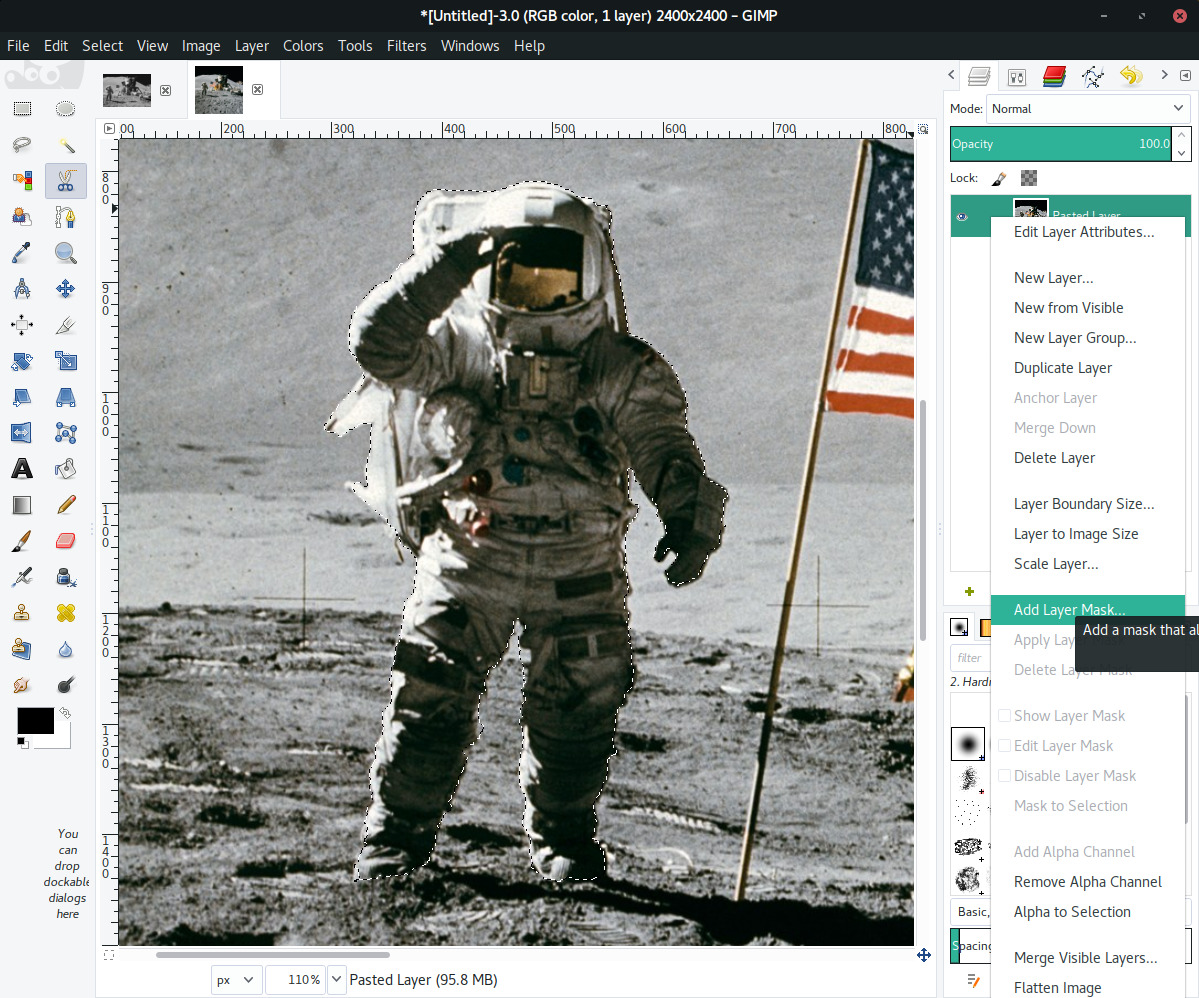
\includegraphics[scale=.15]{Images/mask/mask1}
			\end{figure}
		\end{center}
	\end{frame}

	\begin{frame}{Masques de Fusion}
		Il suffit maintenant de dessiner en noir ou blanc sur le masque de fusion pour faire apparaître (ou disparaitre) certaines zones du calque!
		\begin{itemize}
			\item Blanc $\Longrightarrow $ opaque
			\item Noir $ \Longrightarrow $ transparent
		\end{itemize}
		\begin{center}
			\begin{figure}
				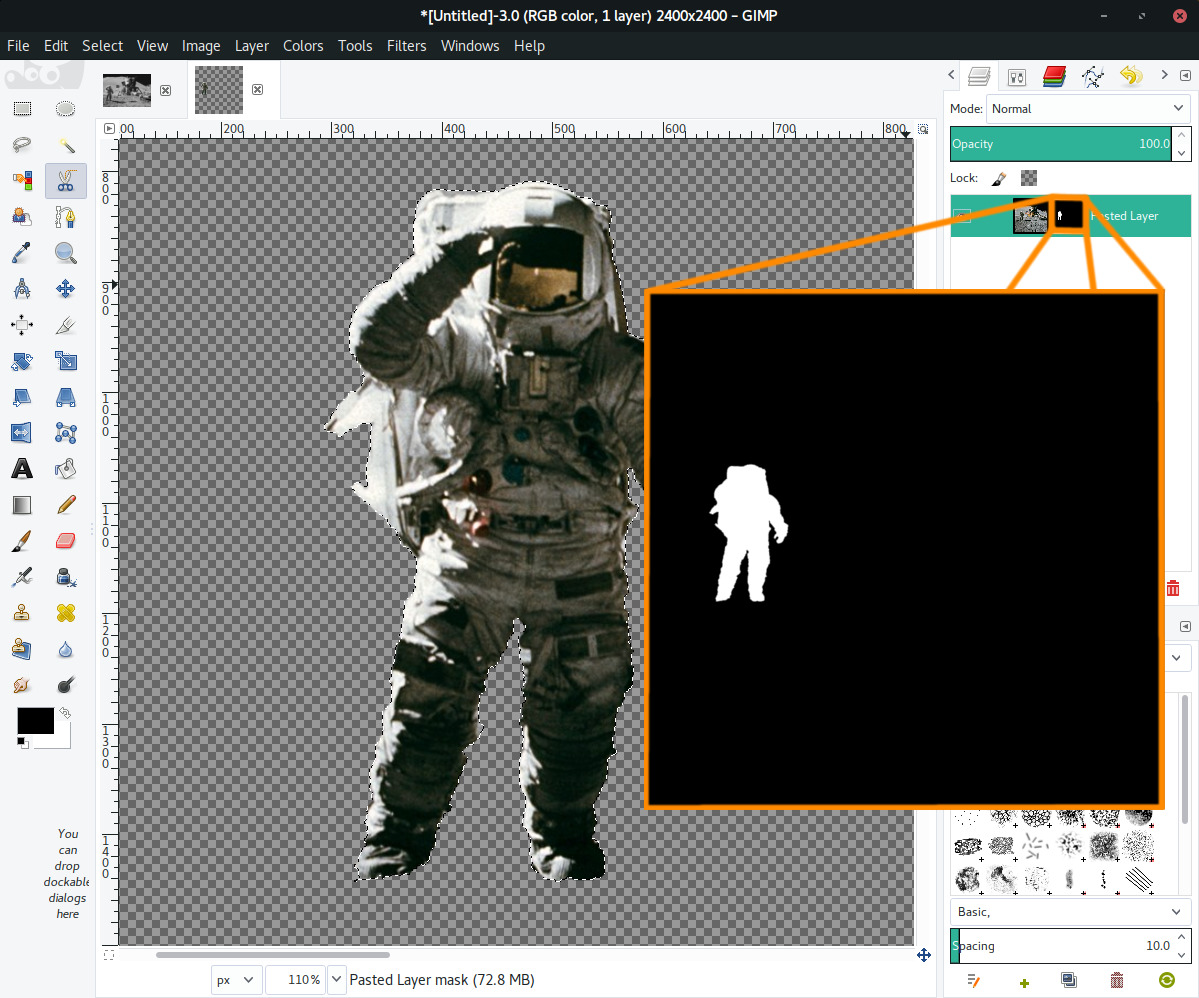
\includegraphics[scale=.15]{Images/mask/mask3}
			\end{figure}
		\end{center}
	\end{frame}

	\begin{frame}{Masques de Fusion}
		"Mais ça a l'air super compliqué! Pourquoi j'utiliserais ça et pas ma gomme?"

		Et bien, pour transformer ceci...

		\begin{figure}[H]
			\centering
			\begin{minipage}{.5\textwidth}
				\centering
				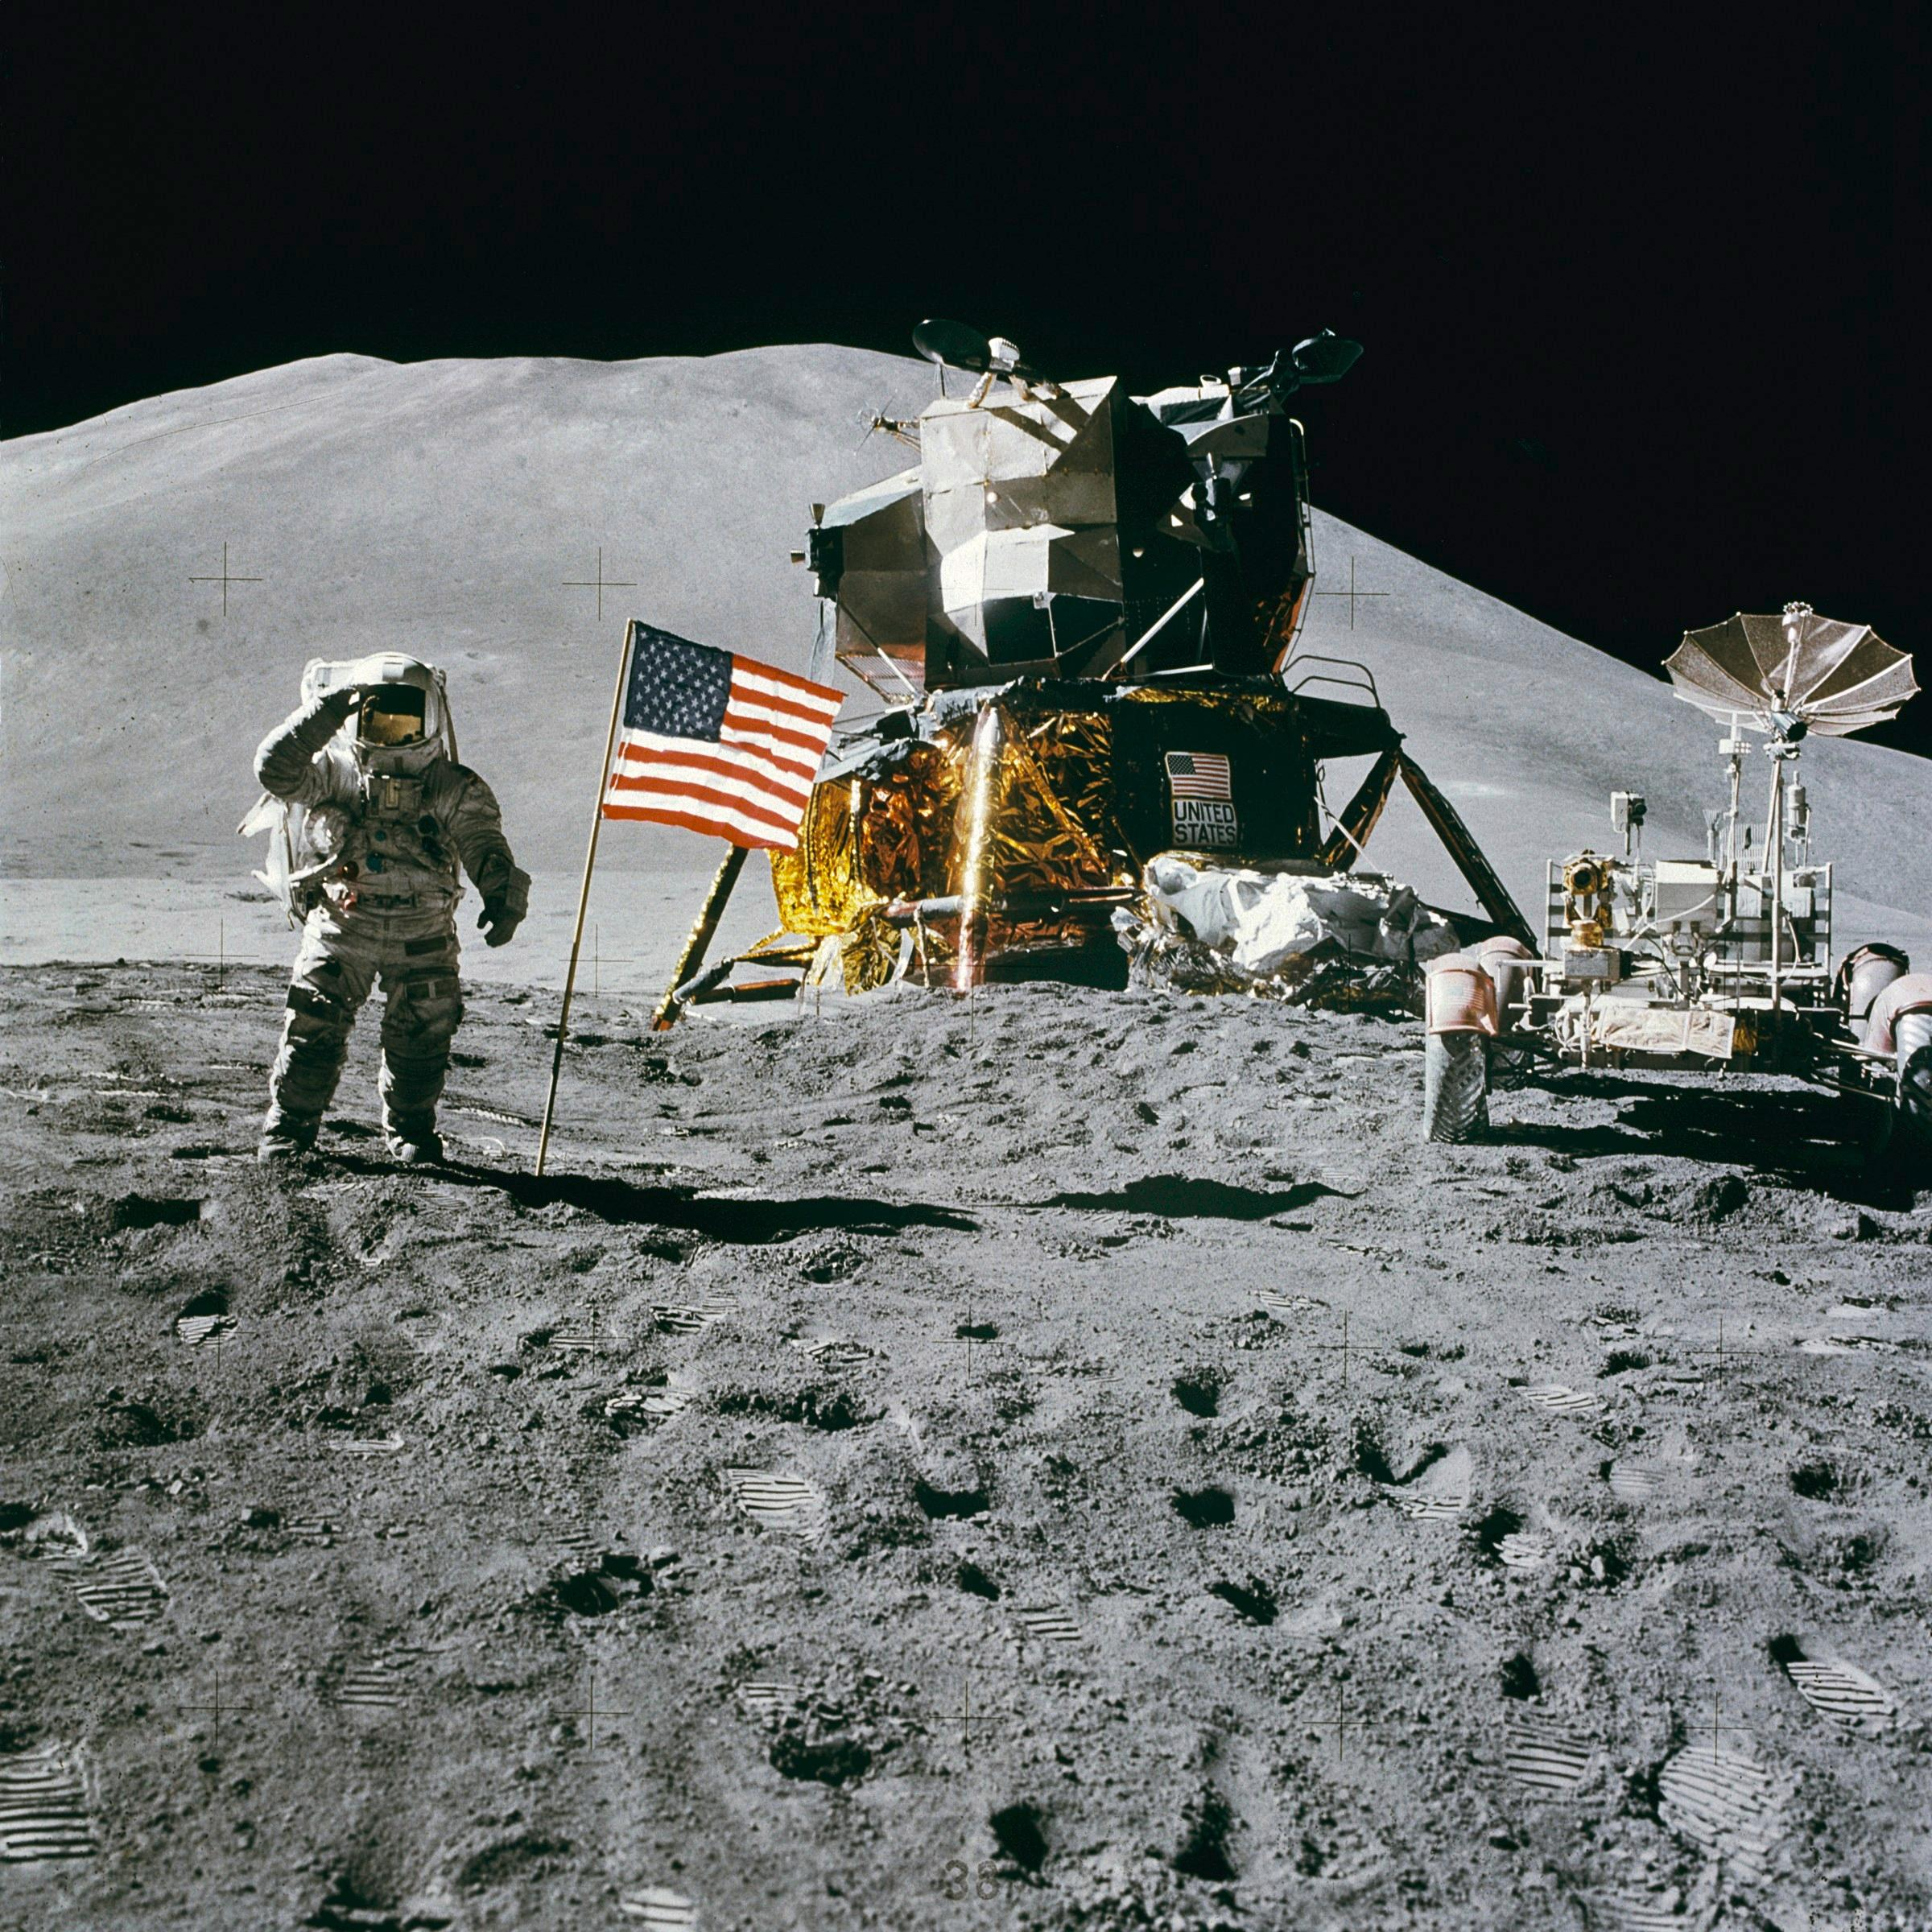
\includegraphics[width=.9\textwidth]{Images/purge/Apollo_15_flag,_rover,_LM,_Irwin}
			\end{minipage}%
			\begin{minipage}{.5\textwidth}
				\centering
				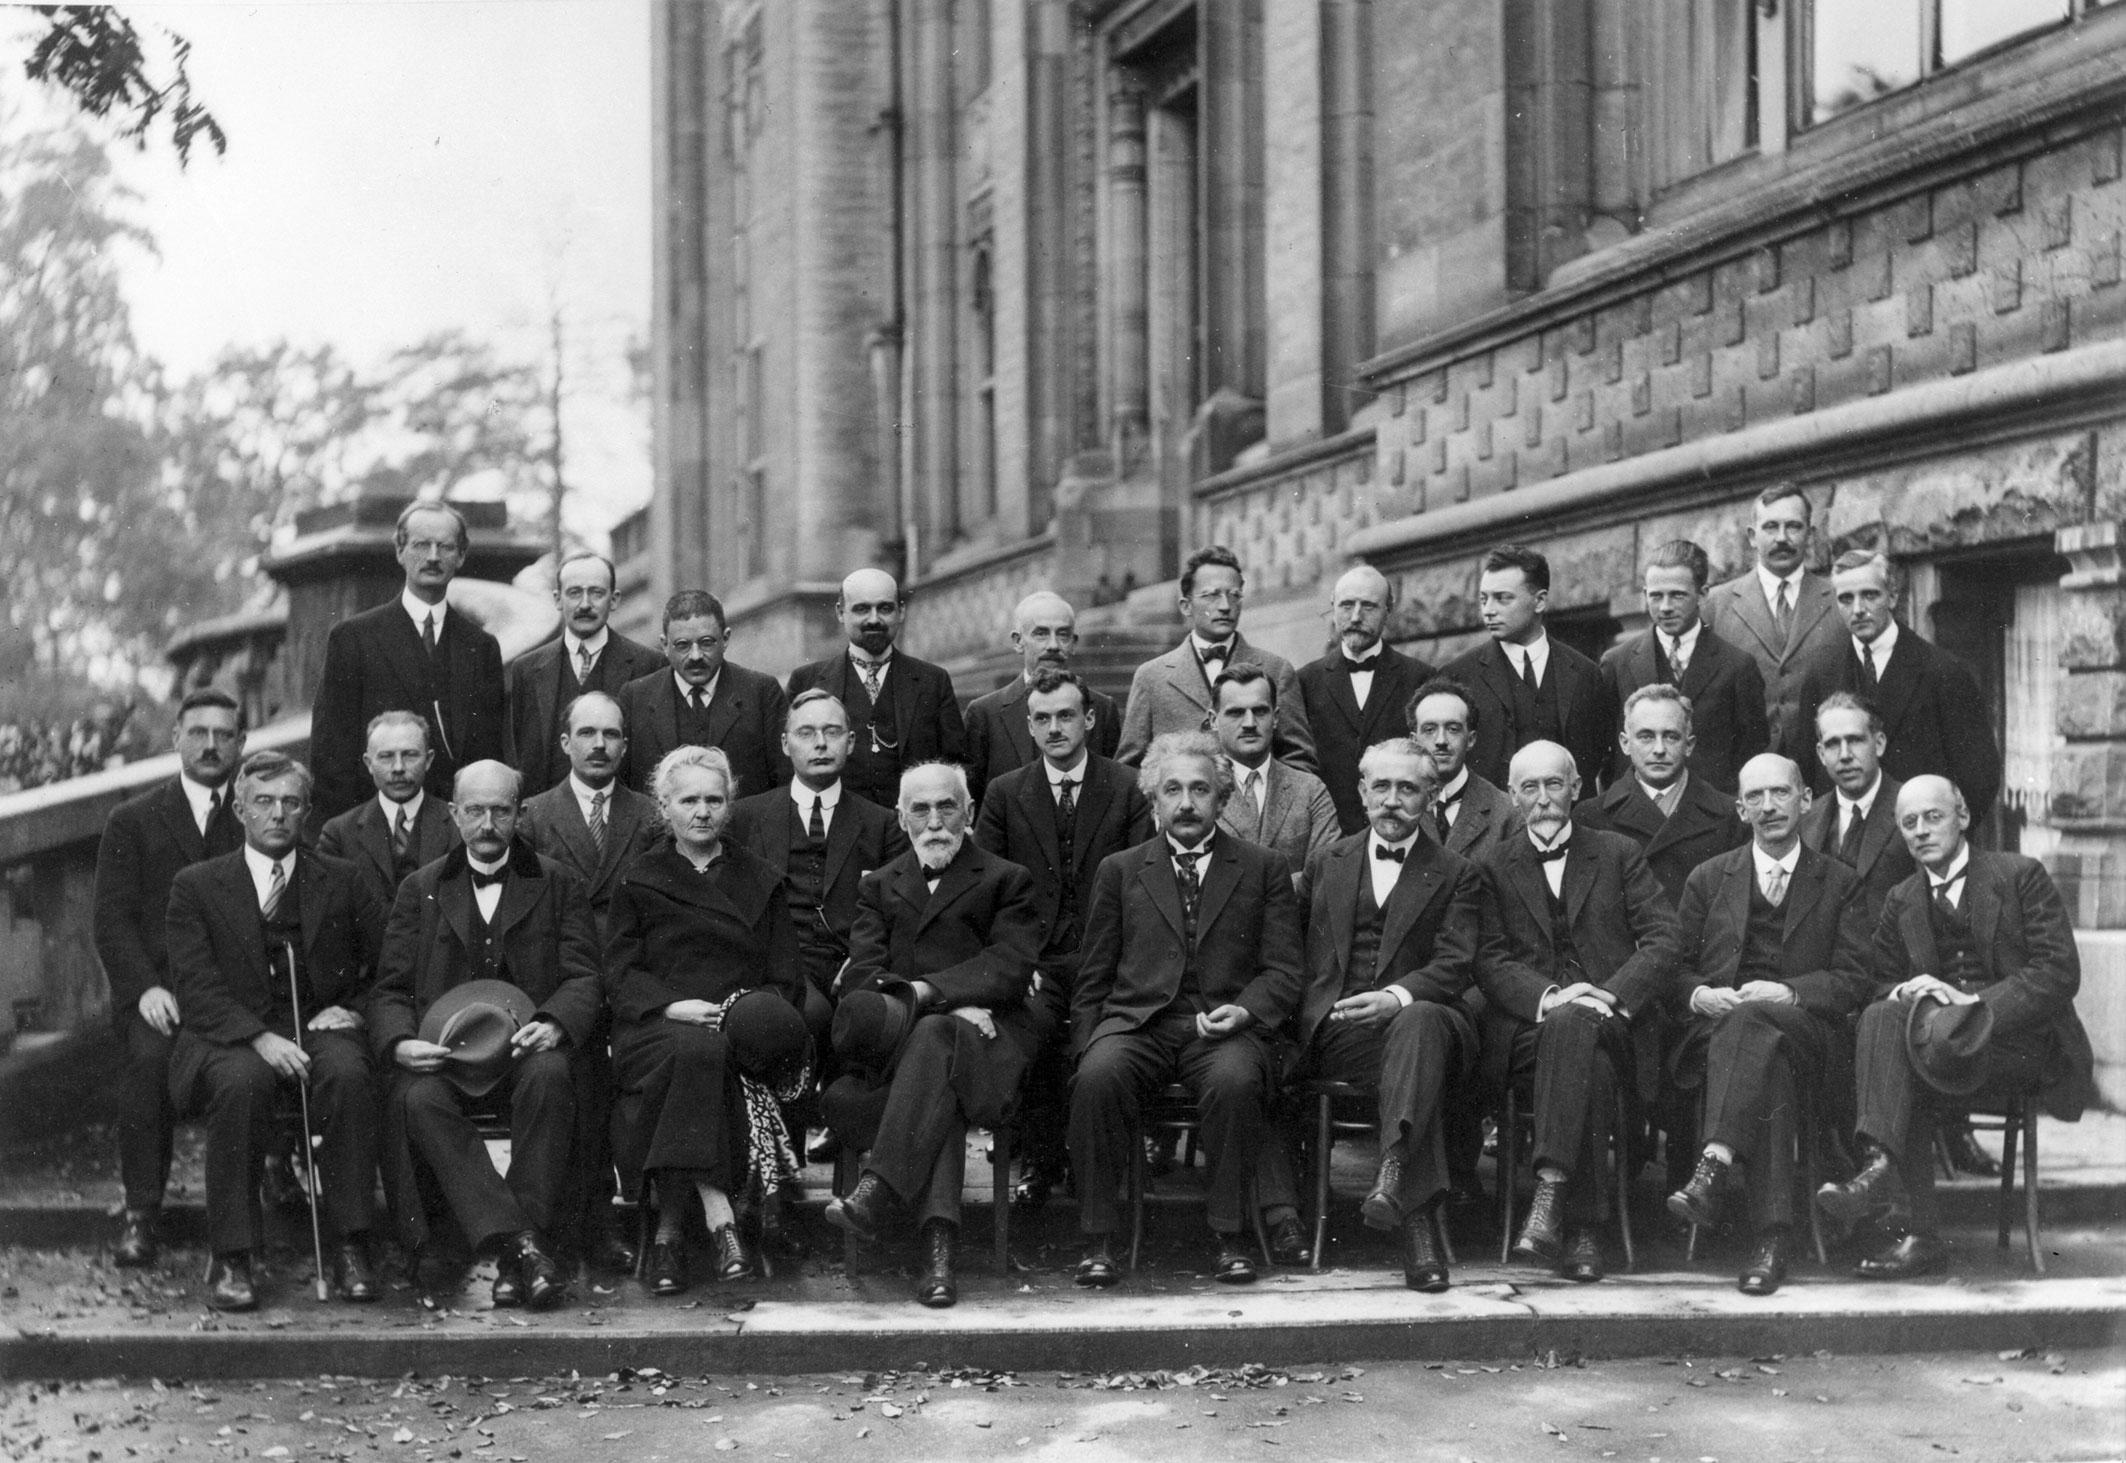
\includegraphics[width=.9\textwidth]{Images/mask/Conference_Solvay_Original}
			\end{minipage}
		\end{figure}


	\end{frame}

	\begin{frame}{Masques de Fusion}
		... En ceci, sans trop se casser la tête car la gomme est "destructive".

		\begin{figure}[H]
			\centering
			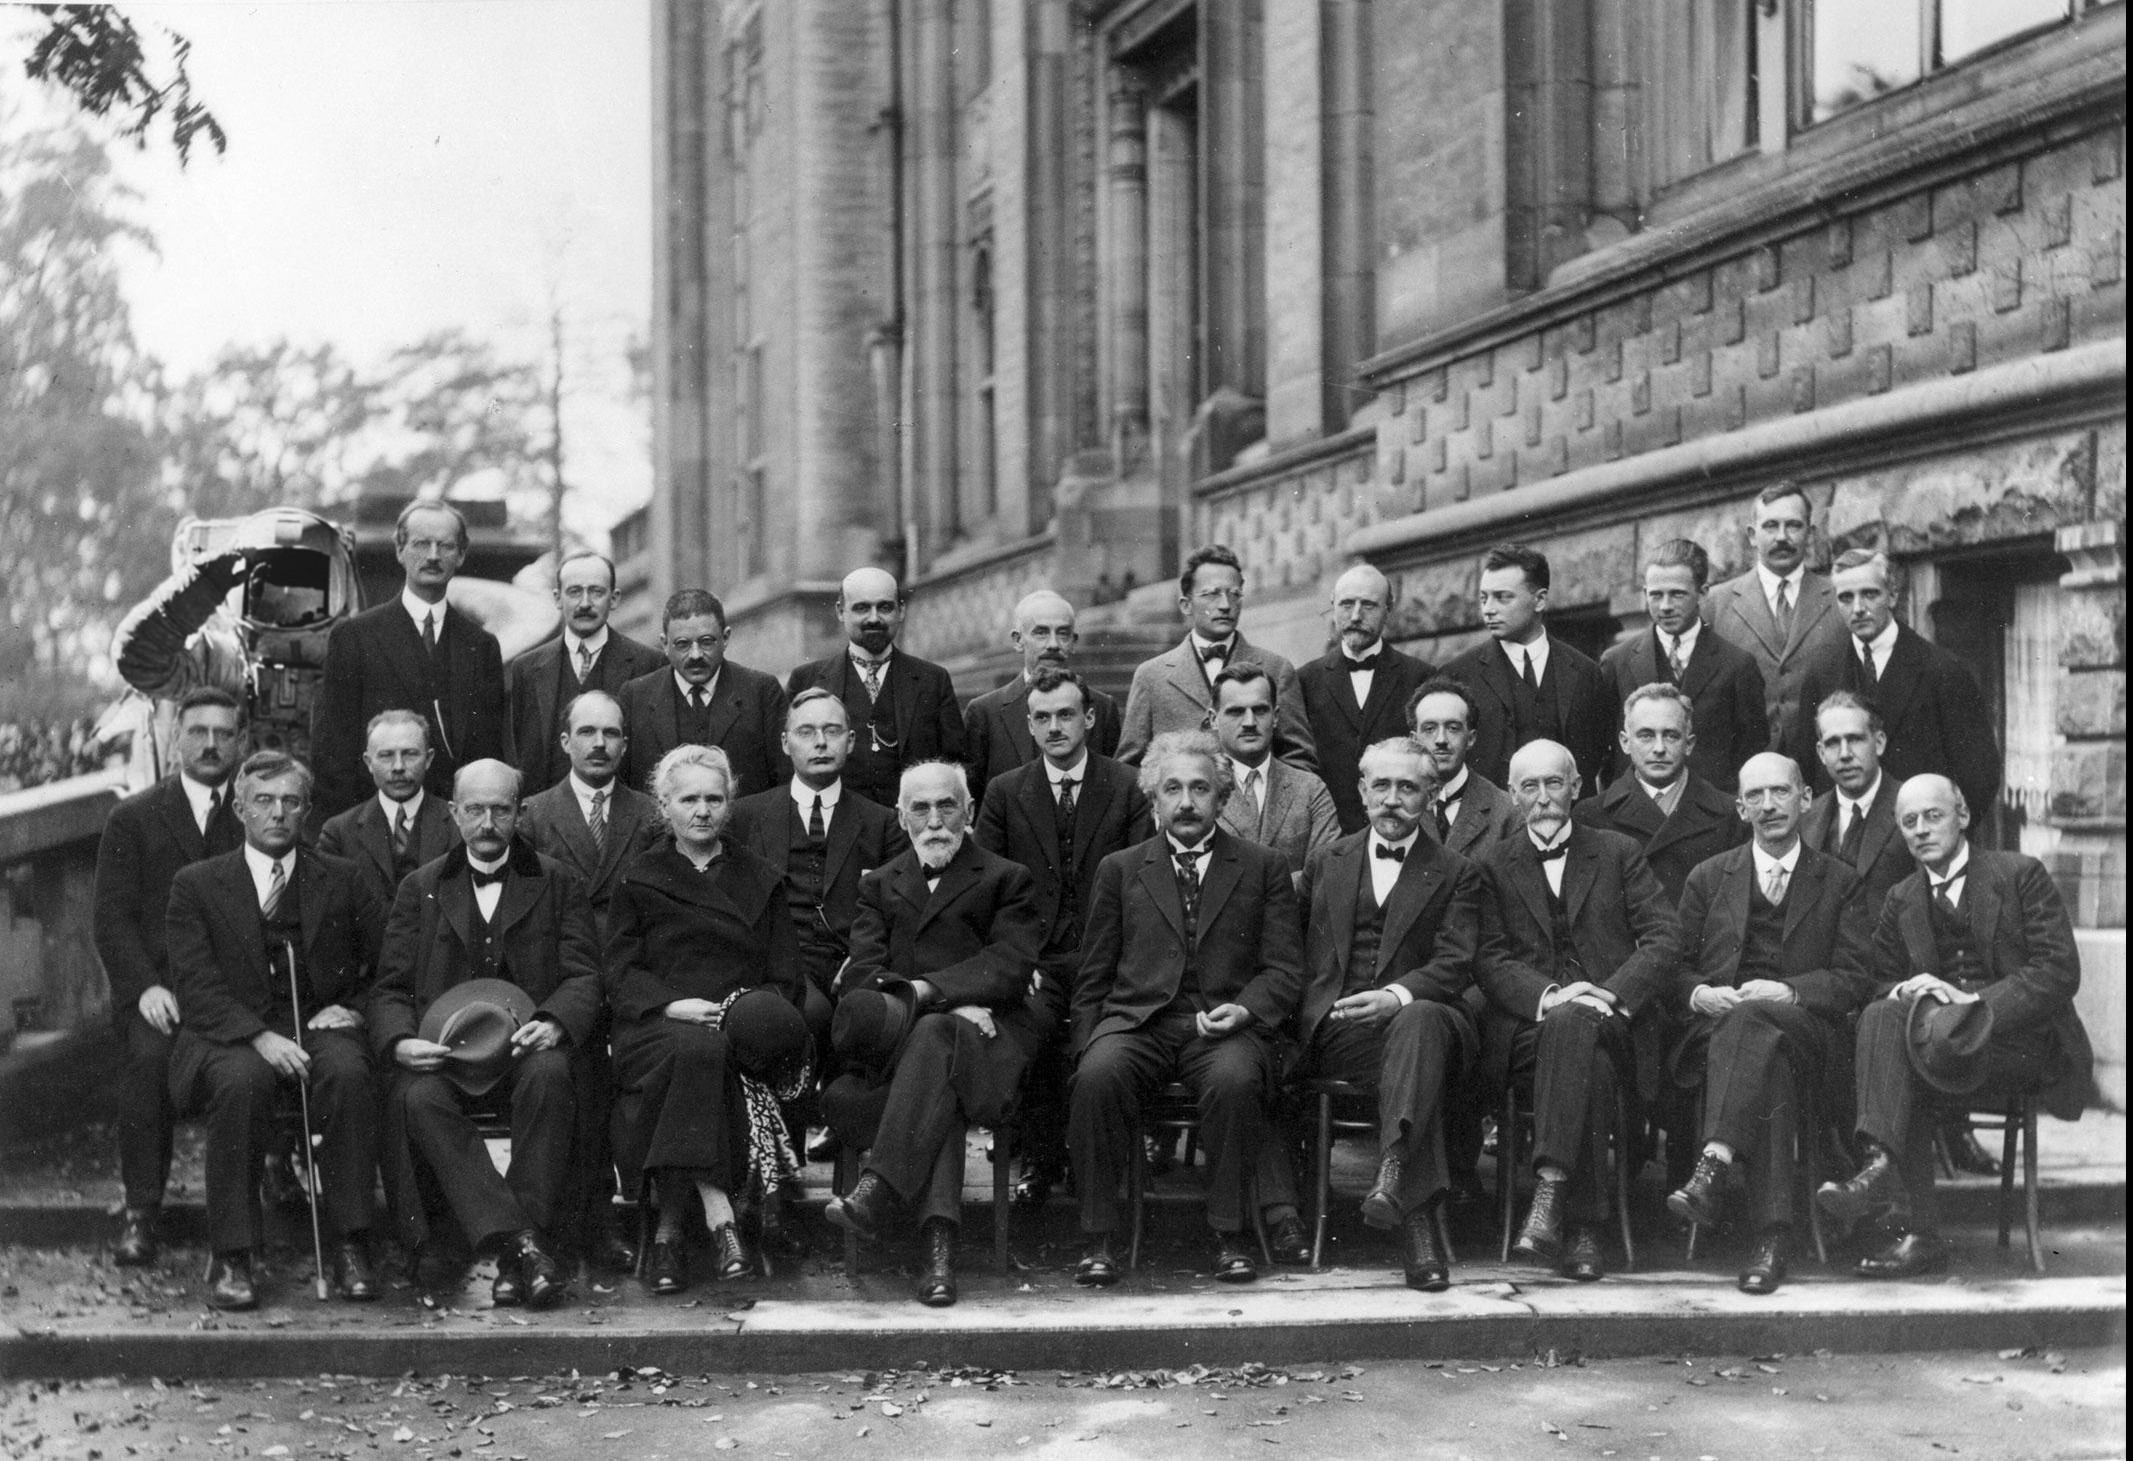
\includegraphics[height=150px]{Images/mask/Conference_Solvay}
			\caption{\scriptsize{1927 Solvay Conference on Quantum Mechanics.}}
		\end{figure}

	\end{frame}



	\begin{frame}{Masques de Fusion}
	\begin{overprint}
	\begin{enumerate}
	\only<1>{
		\framesubtitle{Intégrer un élément dans un image}

		\item[1.] \textbf{Sélectionner} la partie à intégrer et la masquer
		\begin{figure}
		\centering
			\begin{minipage}{.6\textwidth}
				\centering
				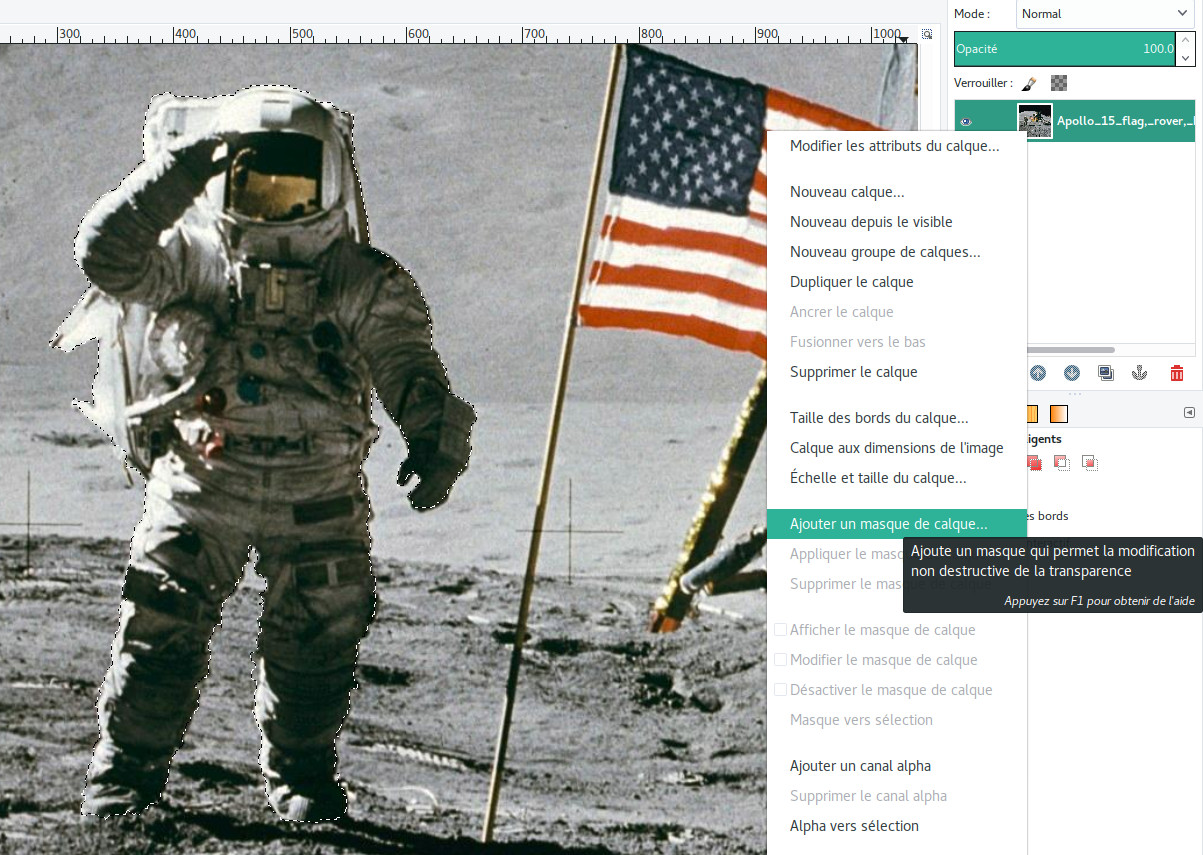
\includegraphics[height=125px]{Images/mask/mask4}
			\end{minipage}%
			\begin{minipage}{.4\textwidth}
				\centering
				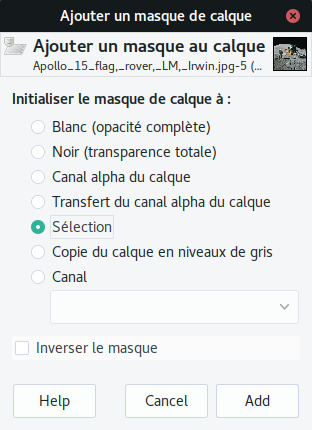
\includegraphics[height=100px]{Images/mask/mask4_2}
			\end{minipage}
		\end{figure}}

	\only<2>{
		\framesubtitle{Intégrer un élément dans un image}

		\item[1.] \textbf{Sélectionner} la partie à intégrer et la masquer
		\begin{figure}
		\centering
		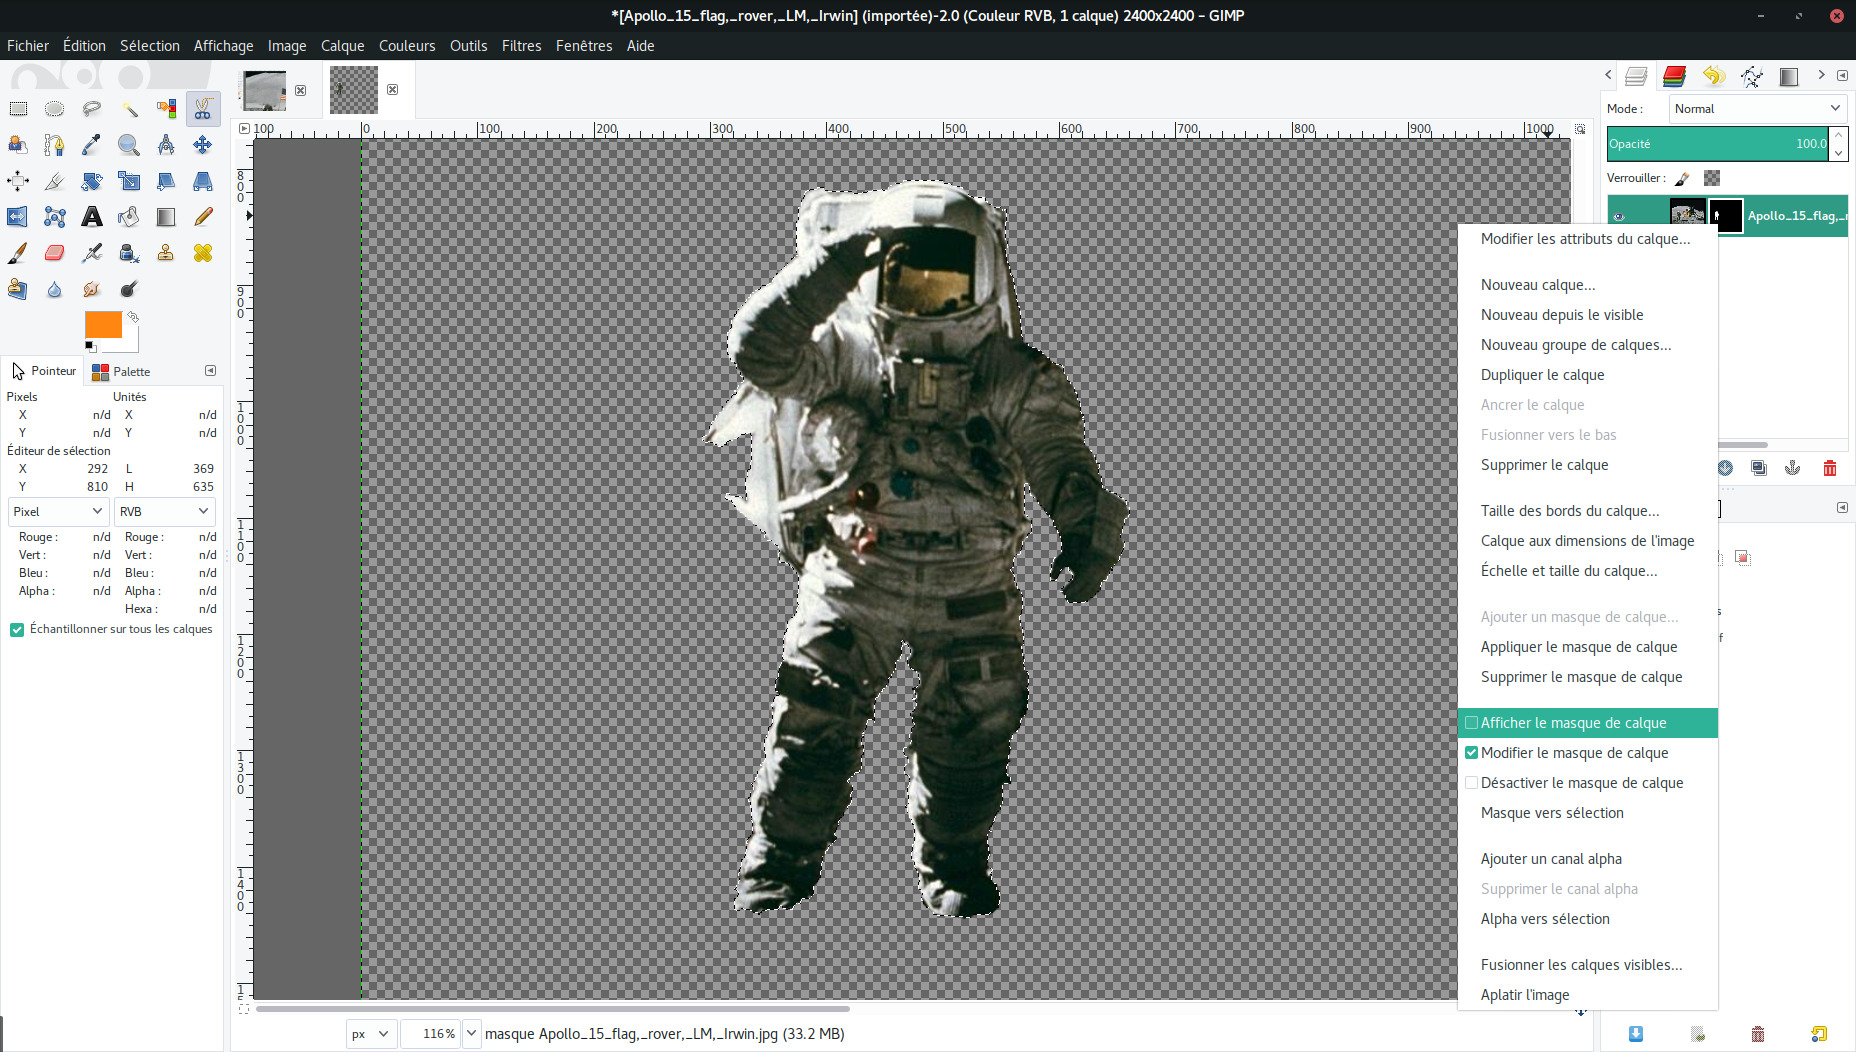
\includegraphics[height=150px]{Images/mask/mask5}
		\end{figure}}

	\only<3>{
		\framesubtitle{Intégrer un élément dans un image}

		\item[1.] \textbf{Sélectionner} la partie à intégrer et la masquer
		\begin{figure}
		\centering
		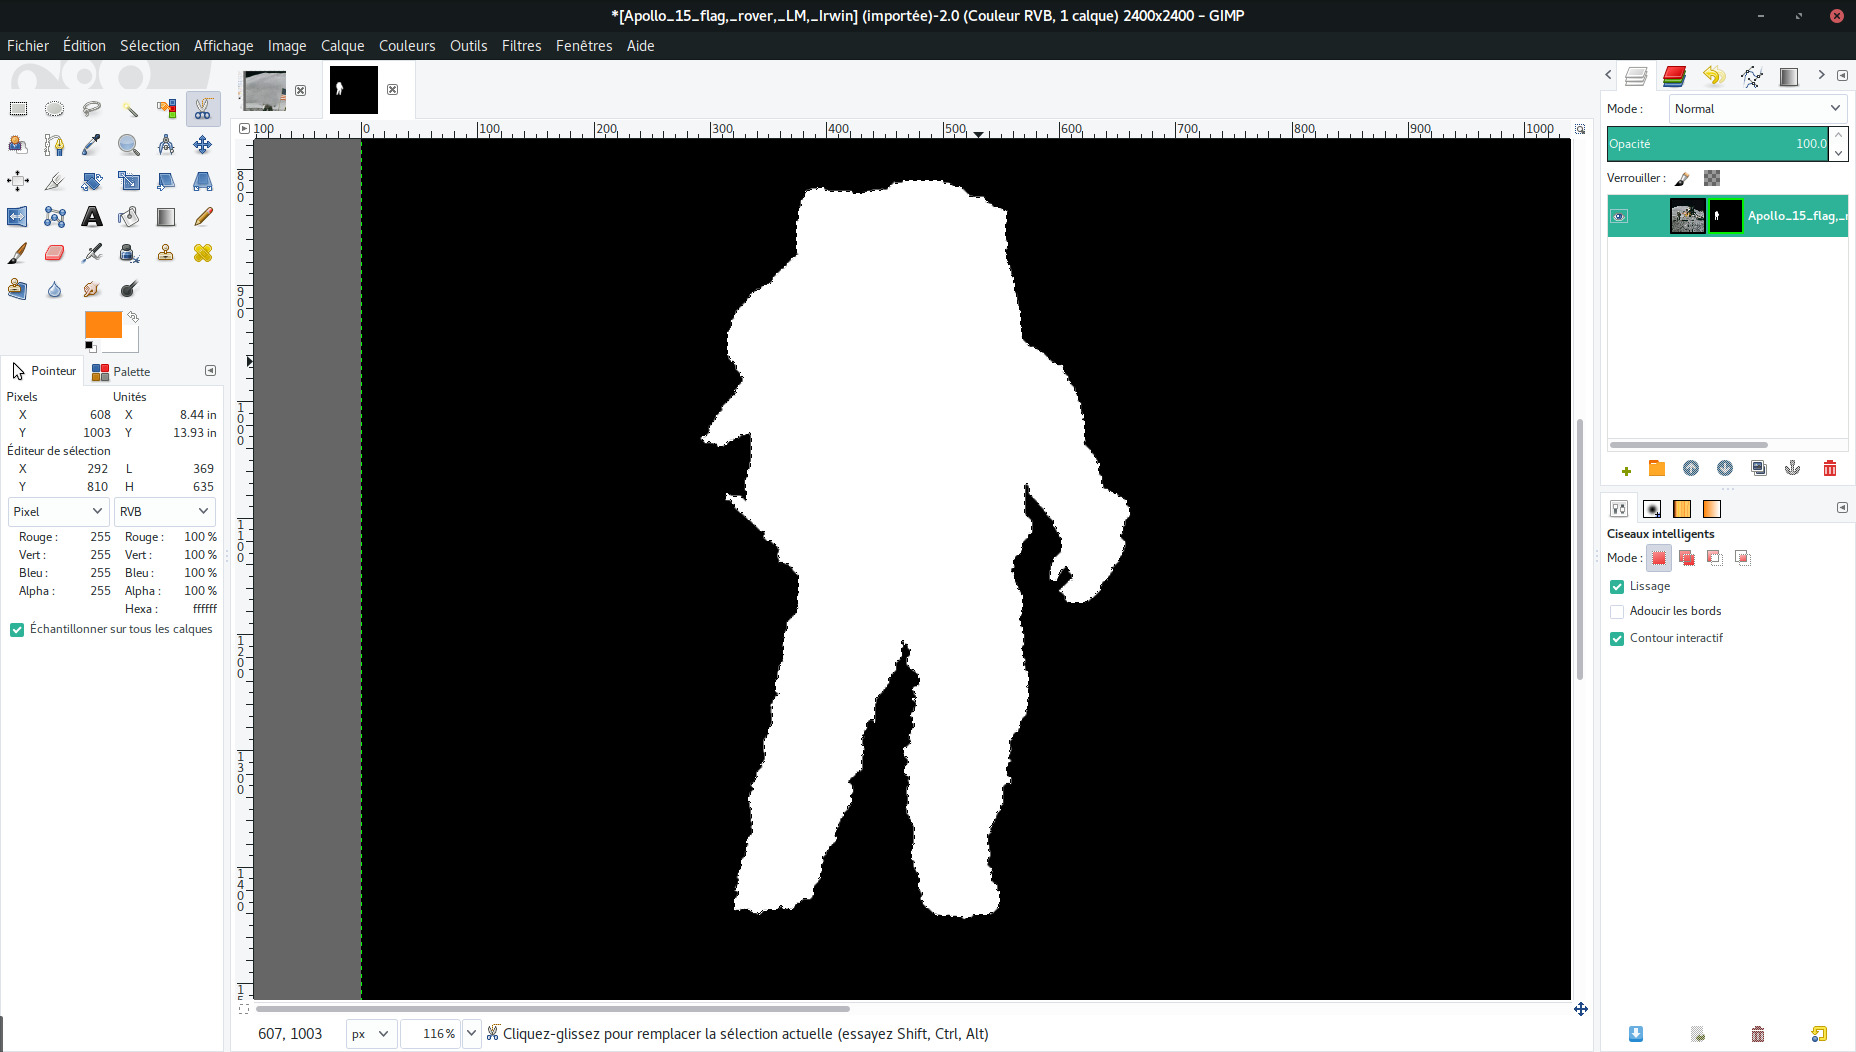
\includegraphics[height=150px]{Images/mask/mask6}
		\end{figure}}

	\only<4>{
		\framesubtitle{Intégrer un élément dans un image}

		\item[2.] \textbf{Déplacer et transformer} l'élément sur l'arrière plan
		\item[3.] \textbf{Sélectionner} les zones qui cacheront notre élément et les noircir sur le masque
		\begin{figure}
		\centering
		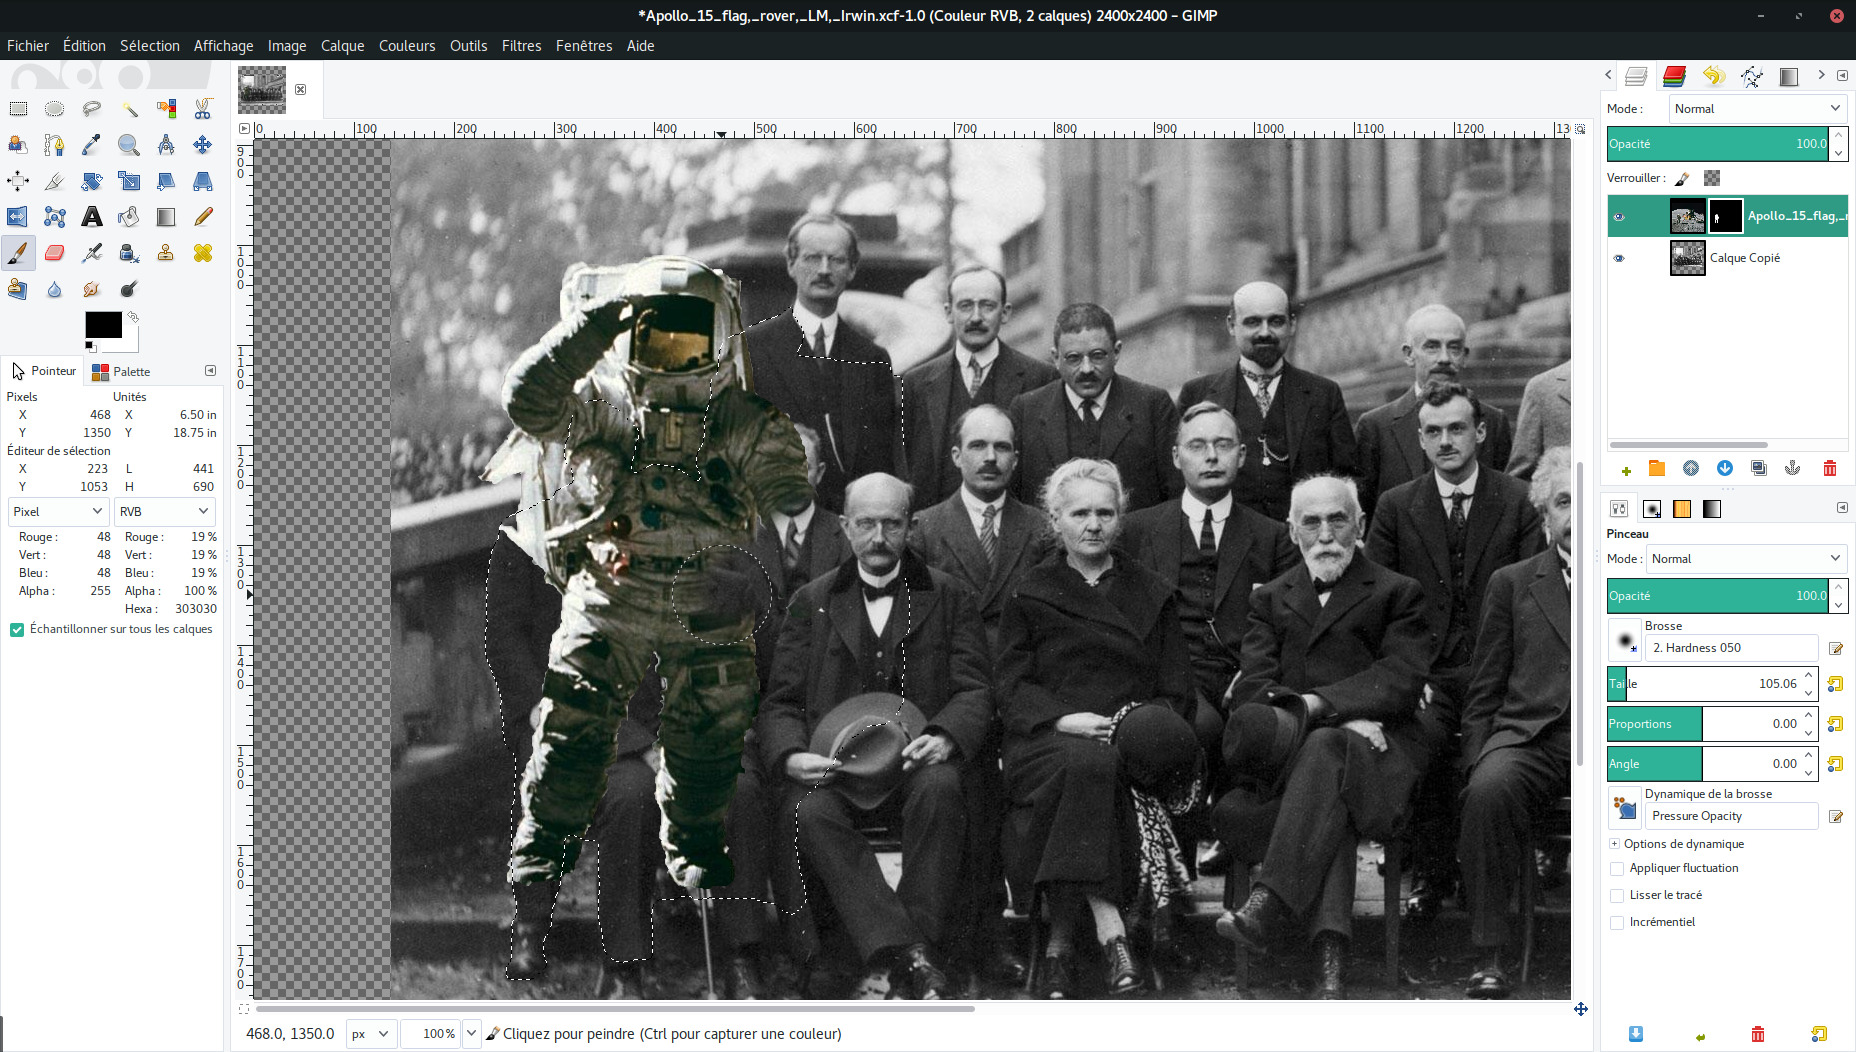
\includegraphics[height=150px]{Images/mask/mask7}
		\end{figure}
	}
	\only<5>{

		\item[4.] \textbf{Améliorer} le contour et régler les couleurs $\rightarrow$ Filtres \& Gestion des Couleurs
			\begin{figure}
		\centering
			\begin{minipage}{.5\textwidth}
				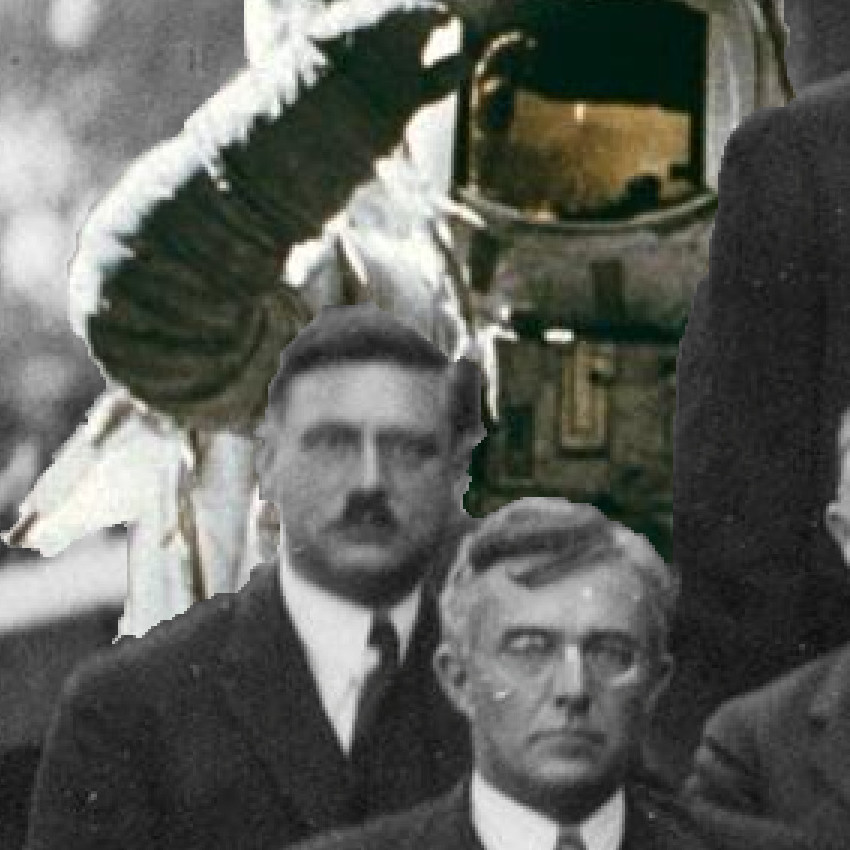
\includegraphics[width=.9\textwidth]{Images/mask/mask8}
			\end{minipage}%
			\begin{minipage}{.5\textwidth}
				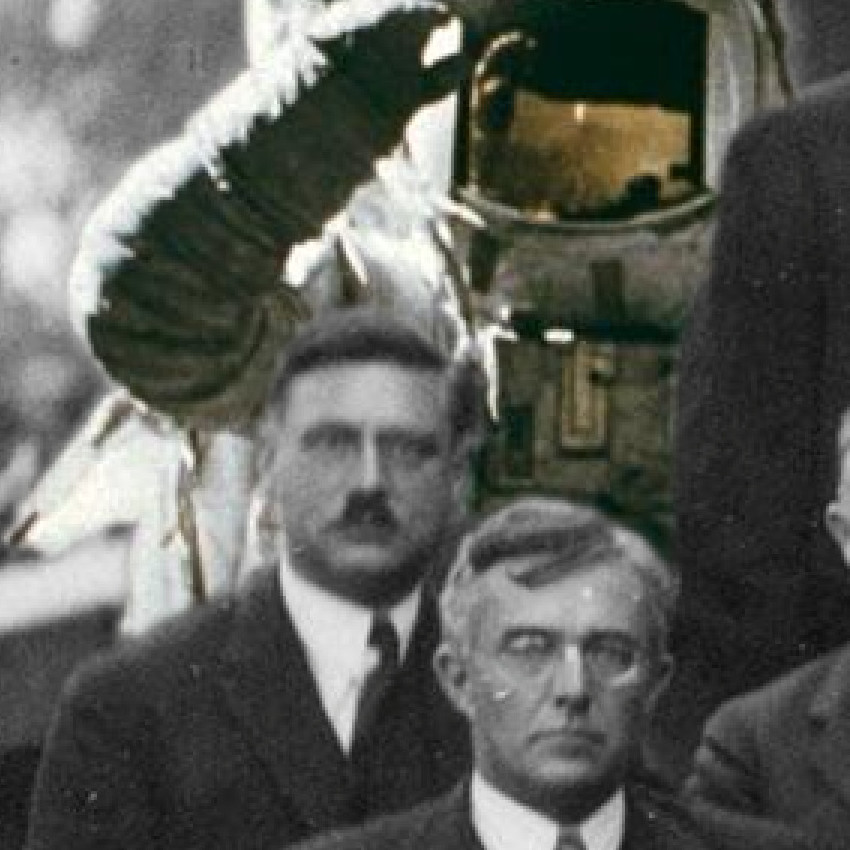
\includegraphics[width=.9\textwidth]{Images/mask/mask8_2}
			\end{minipage}
		\end{figure}
	}





		\end{enumerate}

	\end{overprint}
	\end{frame}

	\begin{frame}{Exercices II}
	\begin{center}
		À vous de jouer ! Faites redescrendre l'astronaute jusqu'à la conférence de Solvay !
		\begin{itemize}
			\item Apollo 15: \href{http://louvainlinux.github.io/atelier-gimp/src/Images/purge/Apollo_15_flag,_rover,_LM,_Irwin.jpg}{Lien de l'image}
			\item Conférence de Solvay: \href{http://louvainlinux.github.io/atelier-gimp/src/Images/mask/Conference_Solvay_Original.jpg}{Lien de l'image}
		\end{itemize}
	\end{center}
	\end{frame}



%% PURGES STALINIENNES %%
	\begin{frame}{Enlever un élément de l'image}
	\begin{enumerate}

	\only<1>{
		\item[1.] \textbf{Dupliquer} le calque pour éviter d'endommager l'original et recouvrir la zone à éliminer avec le tampon de clonage
		\begin{itemize}
			\item Touche \textbf{C}
			\item Touche \textbf{Ctrl} pour sélectionner la zone qui sera clonée
		\end{itemize}
		\begin{center}
			\begin{figure}
				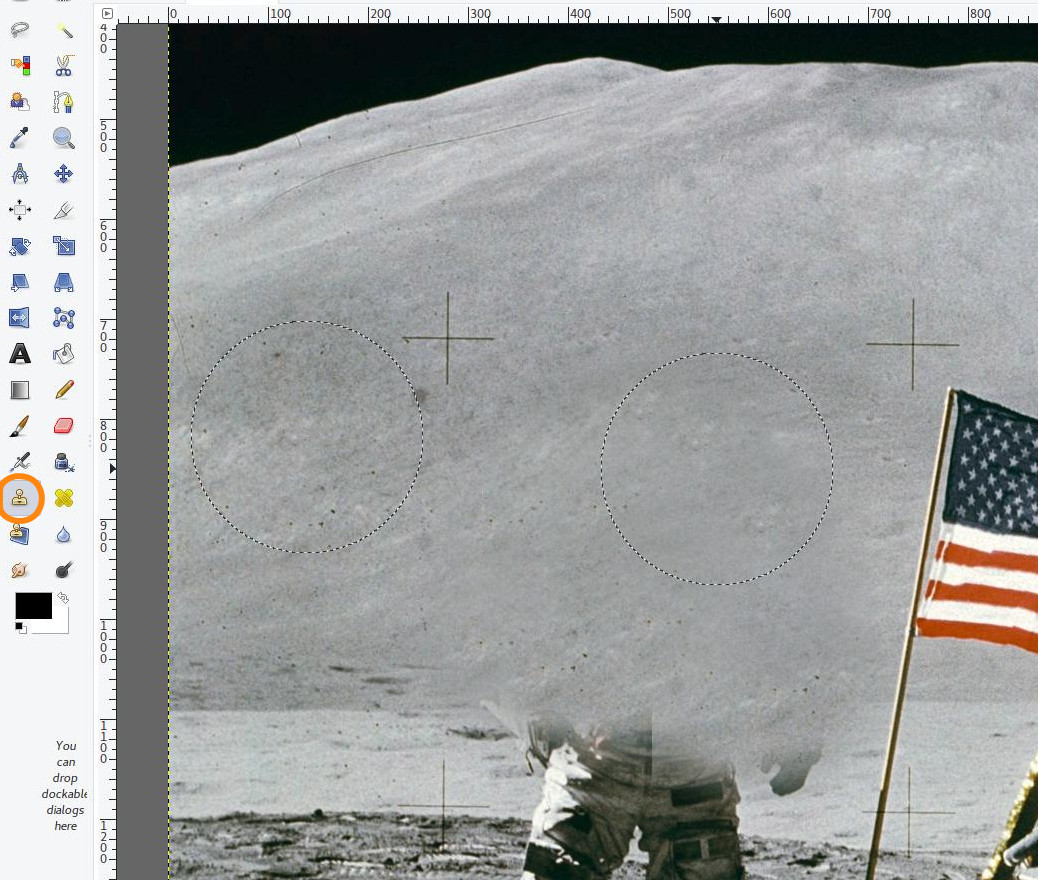
\includegraphics[scale=.15]{Images/purge/purge3}
			\end{figure}
		\end{center}
	}
	\only<2>{

		\item[2.] \textbf{Masquer} le cas échéant et adoucir les transitions avec l'outil correcteur (\textbf{B}). Changer de type de masque de fusion peut aussi s'avérer utile.
		\begin{center}
			\begin{figure}
				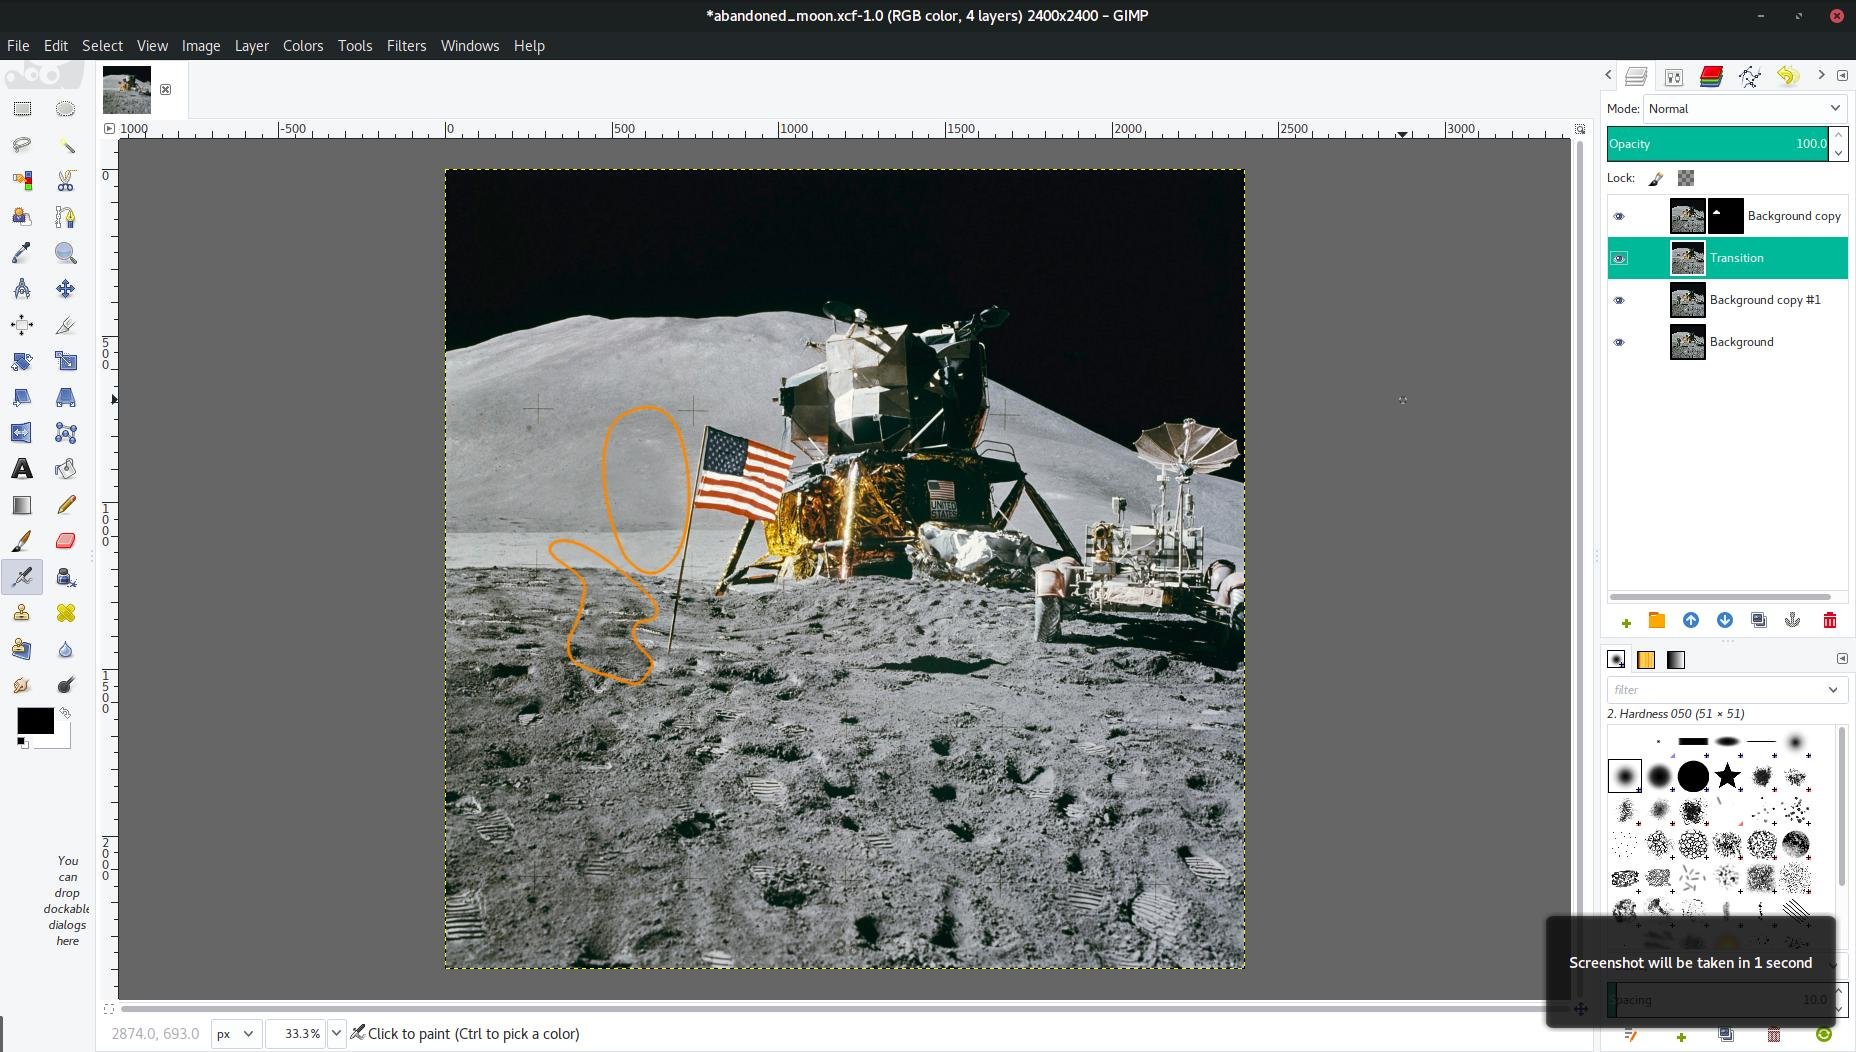
\includegraphics[height=125px]{Images/purge/purge5}
			\end{figure}
		\end{center}
	}

	\end{enumerate}


	\end{frame}
	\begin{frame}{Exercice III}

		\begin{figure}[H]
			\centering
			\begin{minipage}{.5\textwidth}
				\centering
				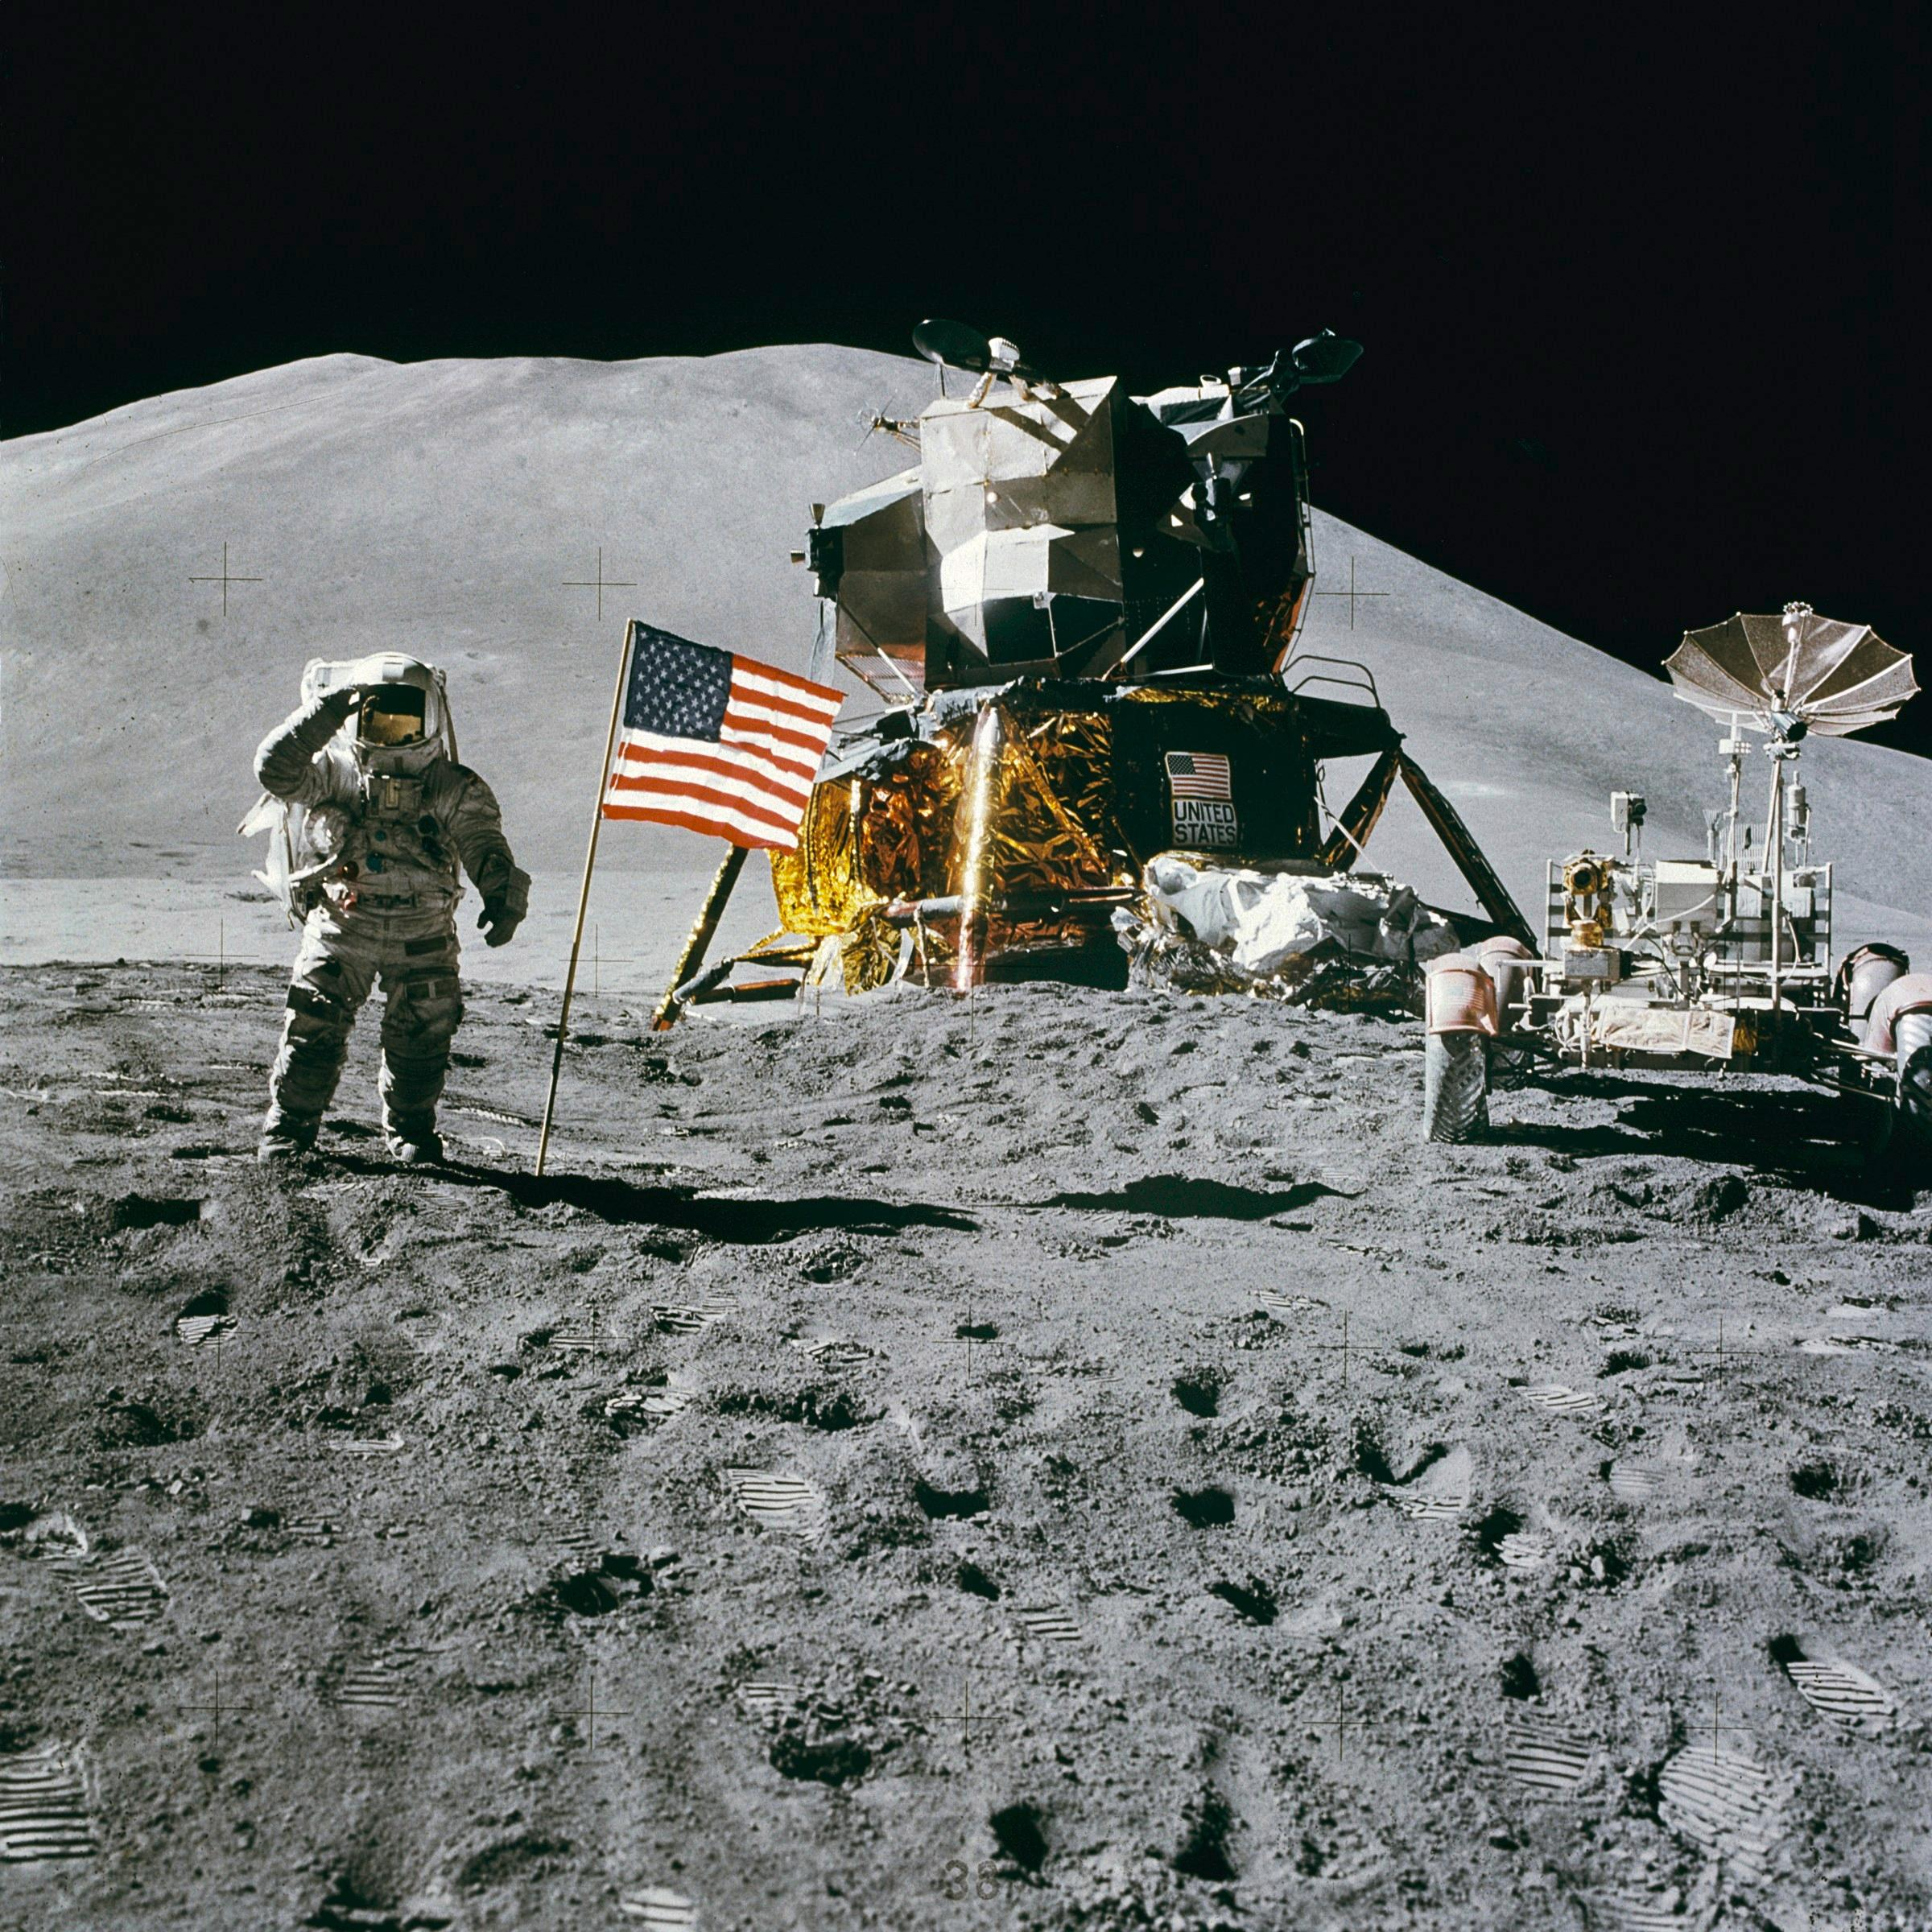
\includegraphics[height=125px]{Images/purge/Apollo_15_flag,_rover,_LM,_Irwin}
				\caption{\tiny{Apollo 15 Lunar Module Pilot James Irwin salutes the U.S. flag.\\\href{http://louvainlinux.github.io/atelier-gimp/src/Images/purge/Apollo_15_flag,_rover,_LM,_Irwin.jpg}{Lien de l'image}}}
			\end{minipage}%
			\begin{minipage}{.5\textwidth}
				\centering
				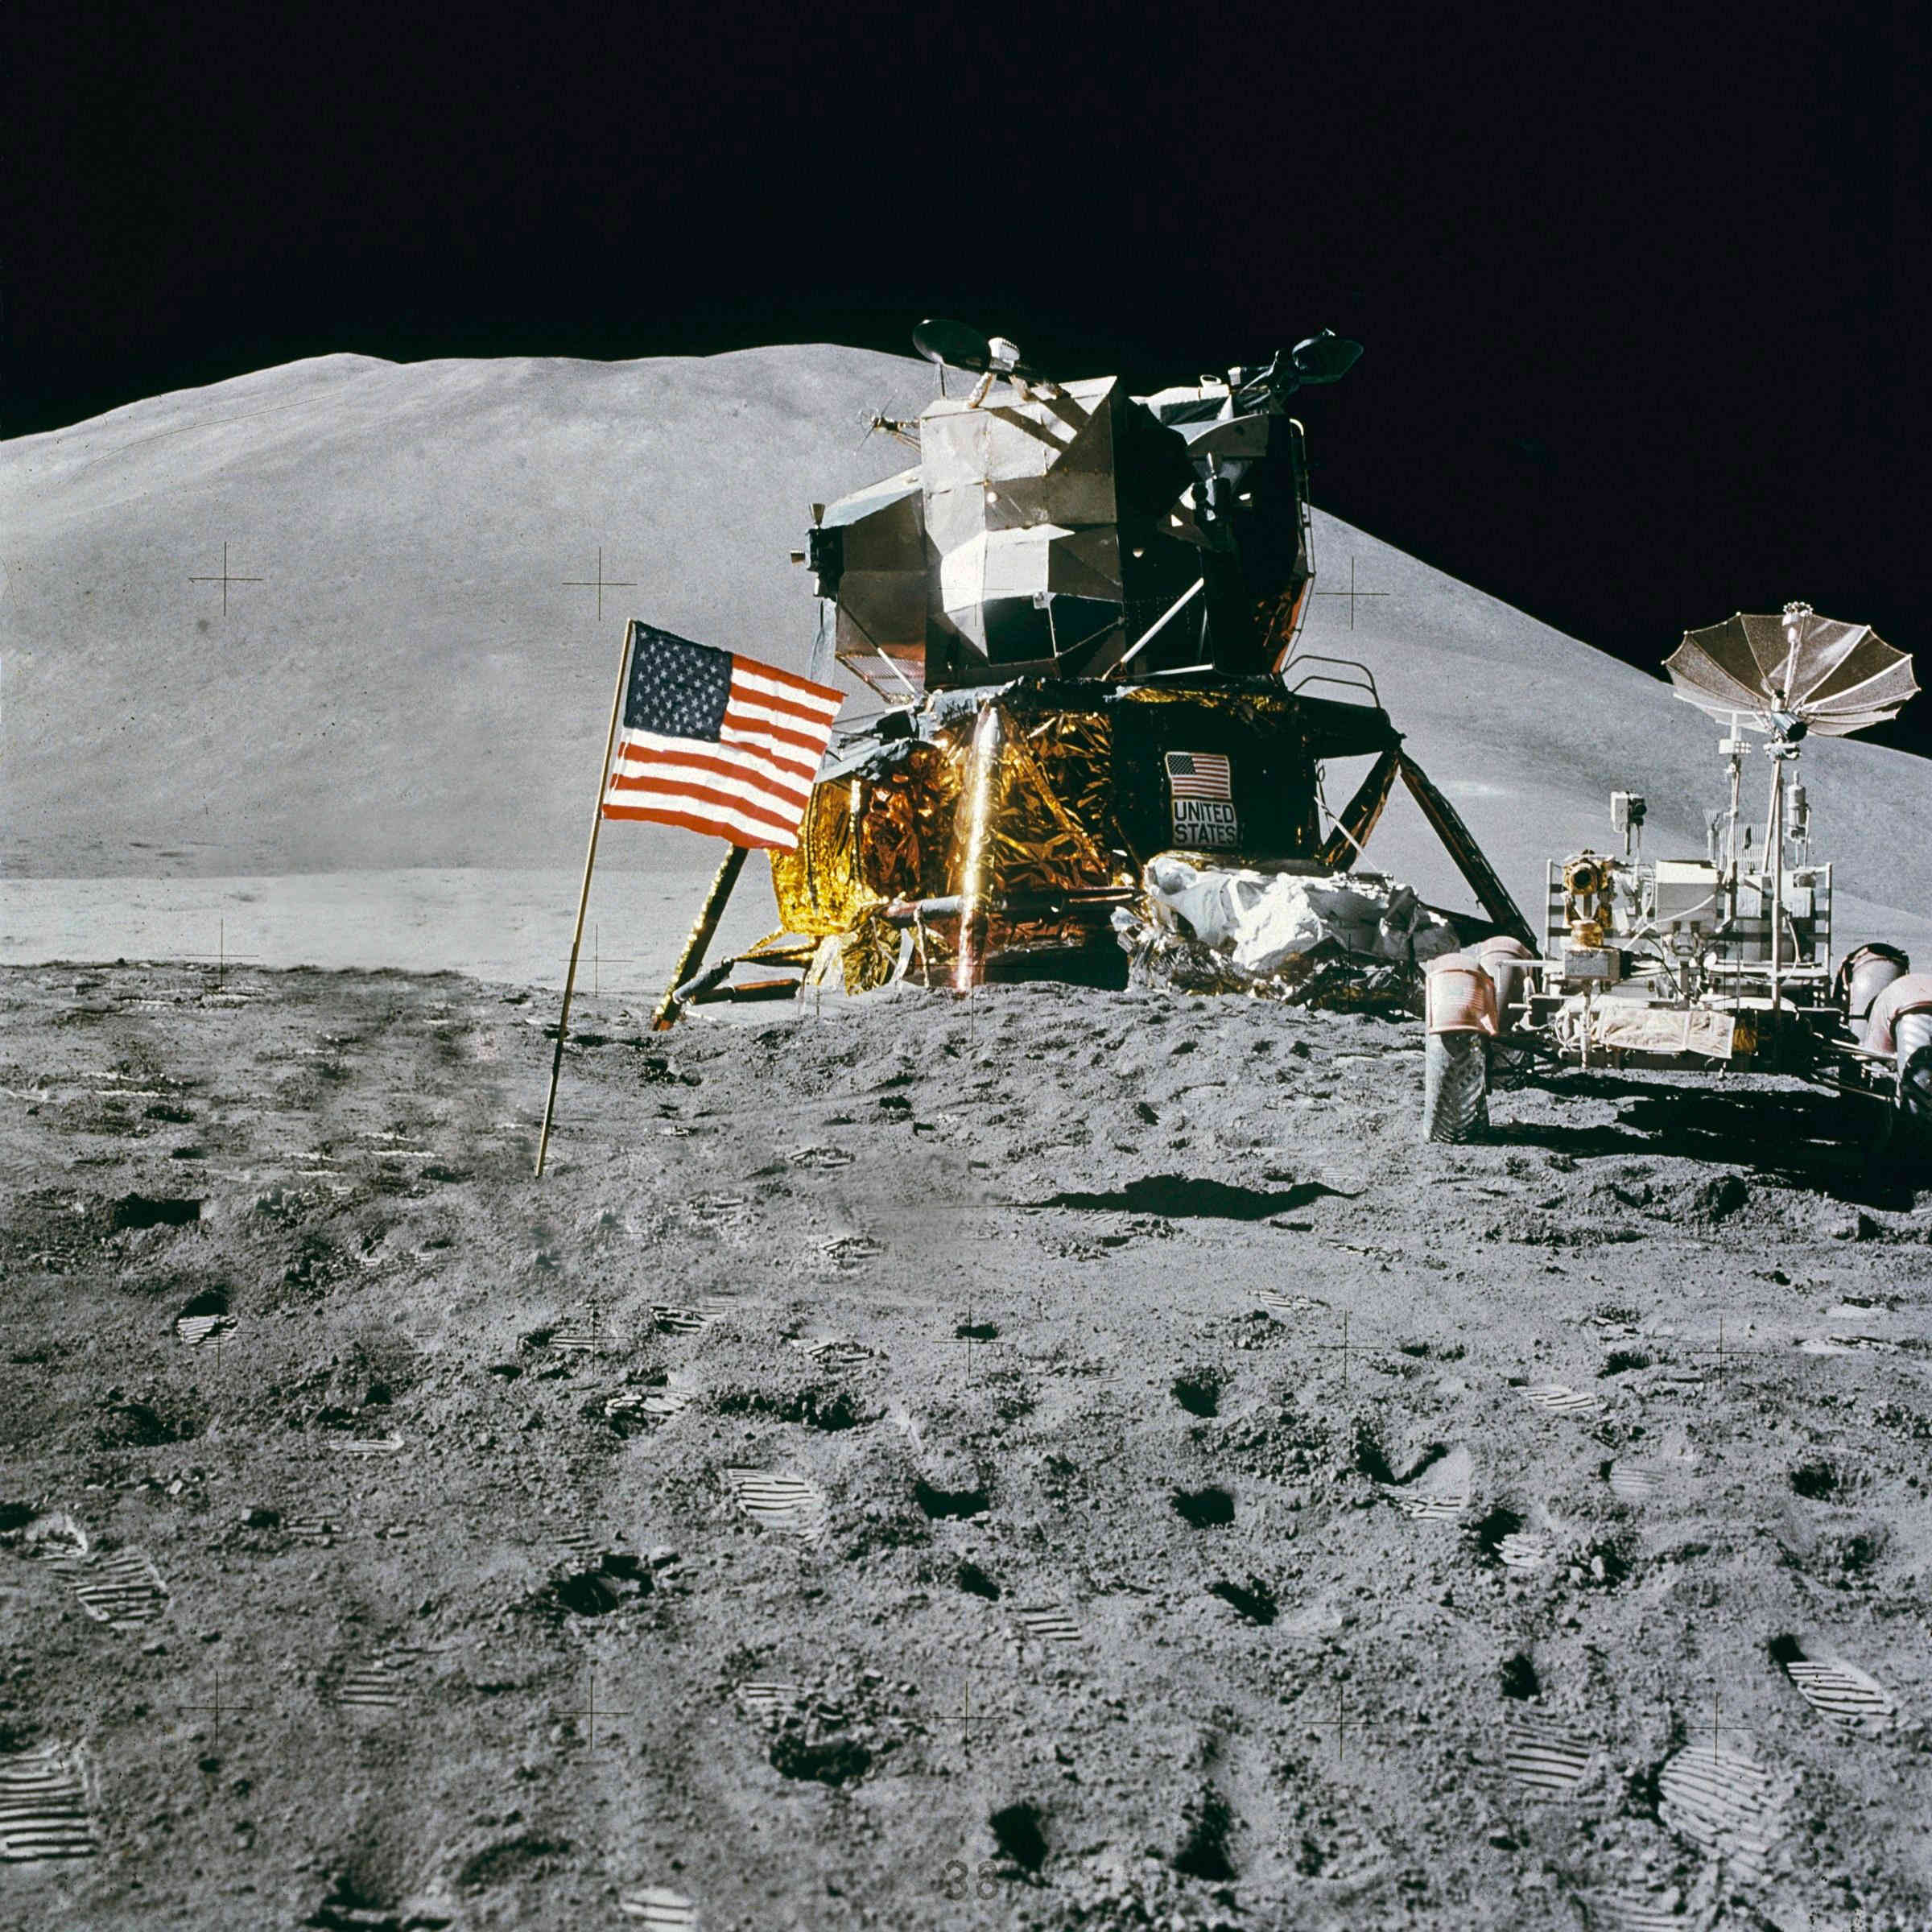
\includegraphics[height=125px]{Images/purge/Apollo_15_flag,_rover,_LM}
				\caption{\tiny{Apollo 15 Lunar Module without James Irwin}}
			\end{minipage}
		\end{figure}
	\end{frame}
